\documentclass[a4paper,twoside,kulak]{kulakreport} %options: kul or kulak (default)

\usepackage[utf8]{inputenc}
\usepackage[dutch]{babel}
\usepackage{eurosym}
\usepackage[utf8]{inputenc}
\usepackage[dutch]{babel}
\usepackage{siunitx}
\usepackage{graphicx}
\usepackage{flafter}
\usepackage{pdfpages}
\usepackage{caption}
\usepackage{subcaption}
\usepackage{booktabs}
\usepackage{url}
\usepackage{hyperref}
\usepackage{gensymb}
\usepackage{tabularx,pbox}




\faculty{Wetenschap \& Technologie Kulak}
\group{Ingenieurswetenschappen}
\title{Handleiding \textit{automated microplate dispenser}}
\author{Team ELISA}
\institute{Matthias Derez, Maxime Dujardin, Korneel Verkens, Seppe Vilain}
\date{Academiejaar 2019 -- 2020}
\address{
	KU Leuven Kulak           \\
	Wetenschap \& Technologie \\
	Etienne Sabbelaan 53, 8500 Kortrijk                \\
	
}

\begin{document} % hier begint de eigenlijke inhoud van het document
	
	\titlepage
	

\chapter*{Voorwoord}


Dit is de handleiding voor de \textit{automated microplate dispenser} die door Team ELISA gebouwd werd tijdens het vak 'Probleemoplossen en ontwerpen, deel 3'. In deze handleiding wordt in detail beschreven hoe men de machine moet installeren en gebruiken. Verder worden ook oplossingen uitgelegd voor mogelijke problemen die kunnen opduiken bij het gebruik van de machine.




\chapter*{Installatie}
\section*{Hardware}
\label{sectie hardware}

Het apparaat wordt bediend via een computerscherm en -muis. Het computerscherm wordt via een HDMI-kabel verbonden met de microcontroller in de groene box zoals aangegeven op Figuur \ref{fig:HDMI}. De computermuis wordt verbonden via de USB-aansluiting zoals weergegeven in Figuur \ref{fig:USB}. Wanneer het scherm en de muis verbonden zijn met de microcontroller zullen deze automatisch verbinding maken. Het is aan te raden deze aangesloten te laten, om te vermijden dat er bedrading los komt en om slijtage aan het toestel te voorkomen. \\
De zwarte stekker in Figuur \ref{fig:stekker} die uit de groene box komt dient men in een wandcontactdoos te stoppen.
\begin{figure}
	\centering
	\begin{minipage}{.5\textwidth}
		\centering
		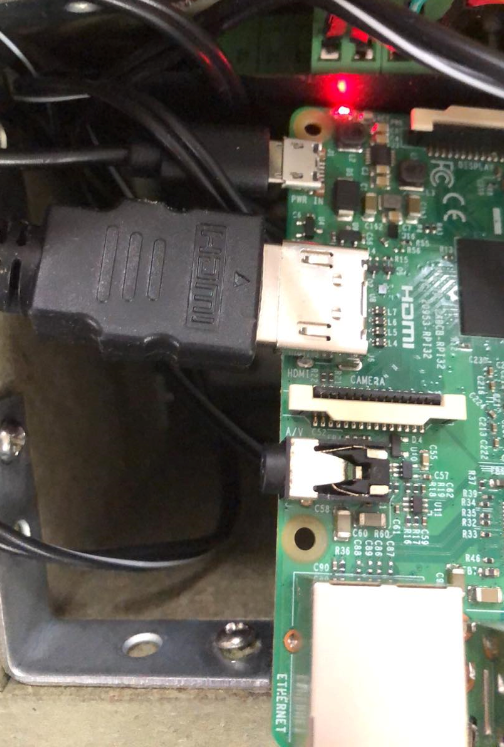
\includegraphics[width=.4\linewidth]{HDMI.png}
		\caption{Aansluiting HDMI-kabel scherm}
		\label{fig:HDMI}
	\end{minipage}%
	\begin{minipage}{.5\textwidth}
		\centering
		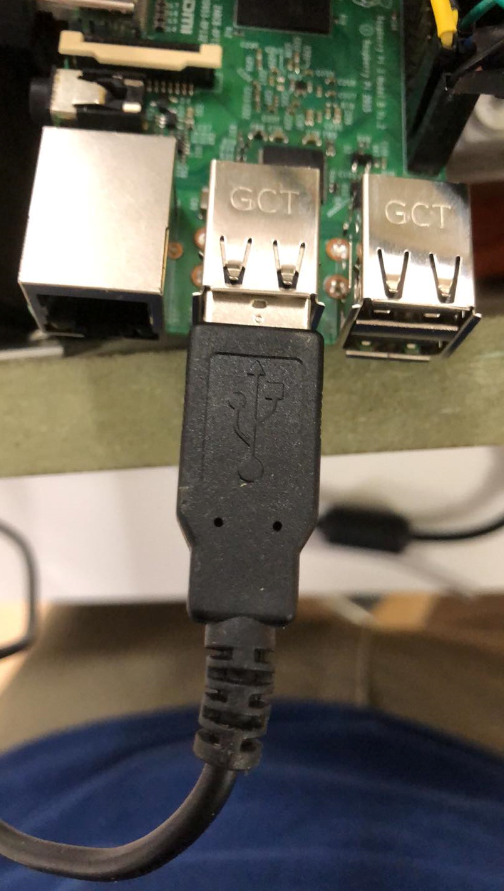
\includegraphics[width=.4\linewidth]{USB.png}
		\caption{Aansluiting USB-kabel muis}
		\label{fig:USB}
	\end{minipage}
\end{figure}
\begin{figure}[h]
	\centering
	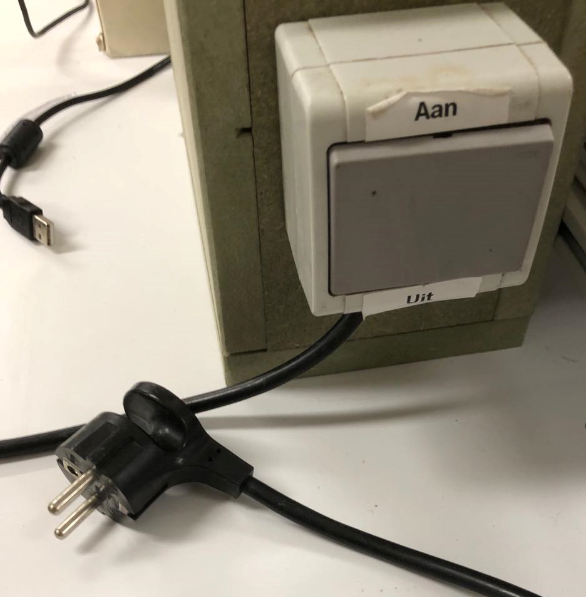
\includegraphics[width=0.5\textwidth]{stekker.png}
	\caption{Zwarte stekker}
	\label{fig:stekker}
	
\end{figure} 



%Om de Automated Microplate Dispenser (verder afgekort als AMD) te kunnen gebruiken, zal men een scherm met hdmi aansluiten en een muis met usb aansluiting nodig hebben. \\
%Deze moet men bevestigen aan de microcontroller, deze bevind zich in de groene box aan 
%de zijkant van de AMD. De hdmi sluit men aan zoals aangeduid op figuur \ref{figuur1} en de muis zoals aangeduid op figuur \ref{figuur2}. \\


%Wanneer deze aangesloten zijn zullen die automatisch verbinden met de microcontroller. Het is aan te raden deze aangesloten te laten, om slijtage te vermijden aan de microcontroller en de AMD zelf. Ook moet men de AMD zelf nog inpluggen in het stopcontact. Uit de groene box loopt een zwarte snoer met een stekker die in het stopcontact moet gestopt worden.\\ \\
%\color{red} hier enkele figuren invoegen dat ze zien wat we bedoelen (ref figuur1 en 2)
%\color{black}
\section*{Vloeistof}

Vooraleer men het toestel opstart, dient men de te gebruiken vloeistof klaar te hebben staan. Er kunnen twee verschillende soorten vloeistof gebruikt worden: men kan namelijk de linkse rij \textit{microplates} vullen met een andere vloeistof dan de rechtse rij. Aan de linker- en rechterkant van het apparaat hangen twee zwarte pompen, deze zijn gelabeld als 'Pomp Links' en 'Pomp Rechts' (zie Figuren \ref{fig: linkerpomp} en \ref{fig: rechterpomp}). Aan beide pompen hangt een plastic leiding bevestigd wiens uiteinden (zie Figuur \ref{fig: uiteinde leiding}) zich aan de rechterkant van de machine bevinden. Indien men ervoor kiest om één vloeistof te gebruiken, plaatst men de uiteinden van beide leidingen in dezelfde erlenmeyer. Indien met twee vloeistoffen wil gewerkt worden, plaatst men beide uiteinden in twee verschillende erlenmeyers. \\ Wanneer vorige stappen correct uitgevoerd zijn, is het toestel klaar voor gebruik.

\begin{figure}
	\centering
	\begin{minipage}{.5\textwidth}
		\centering
		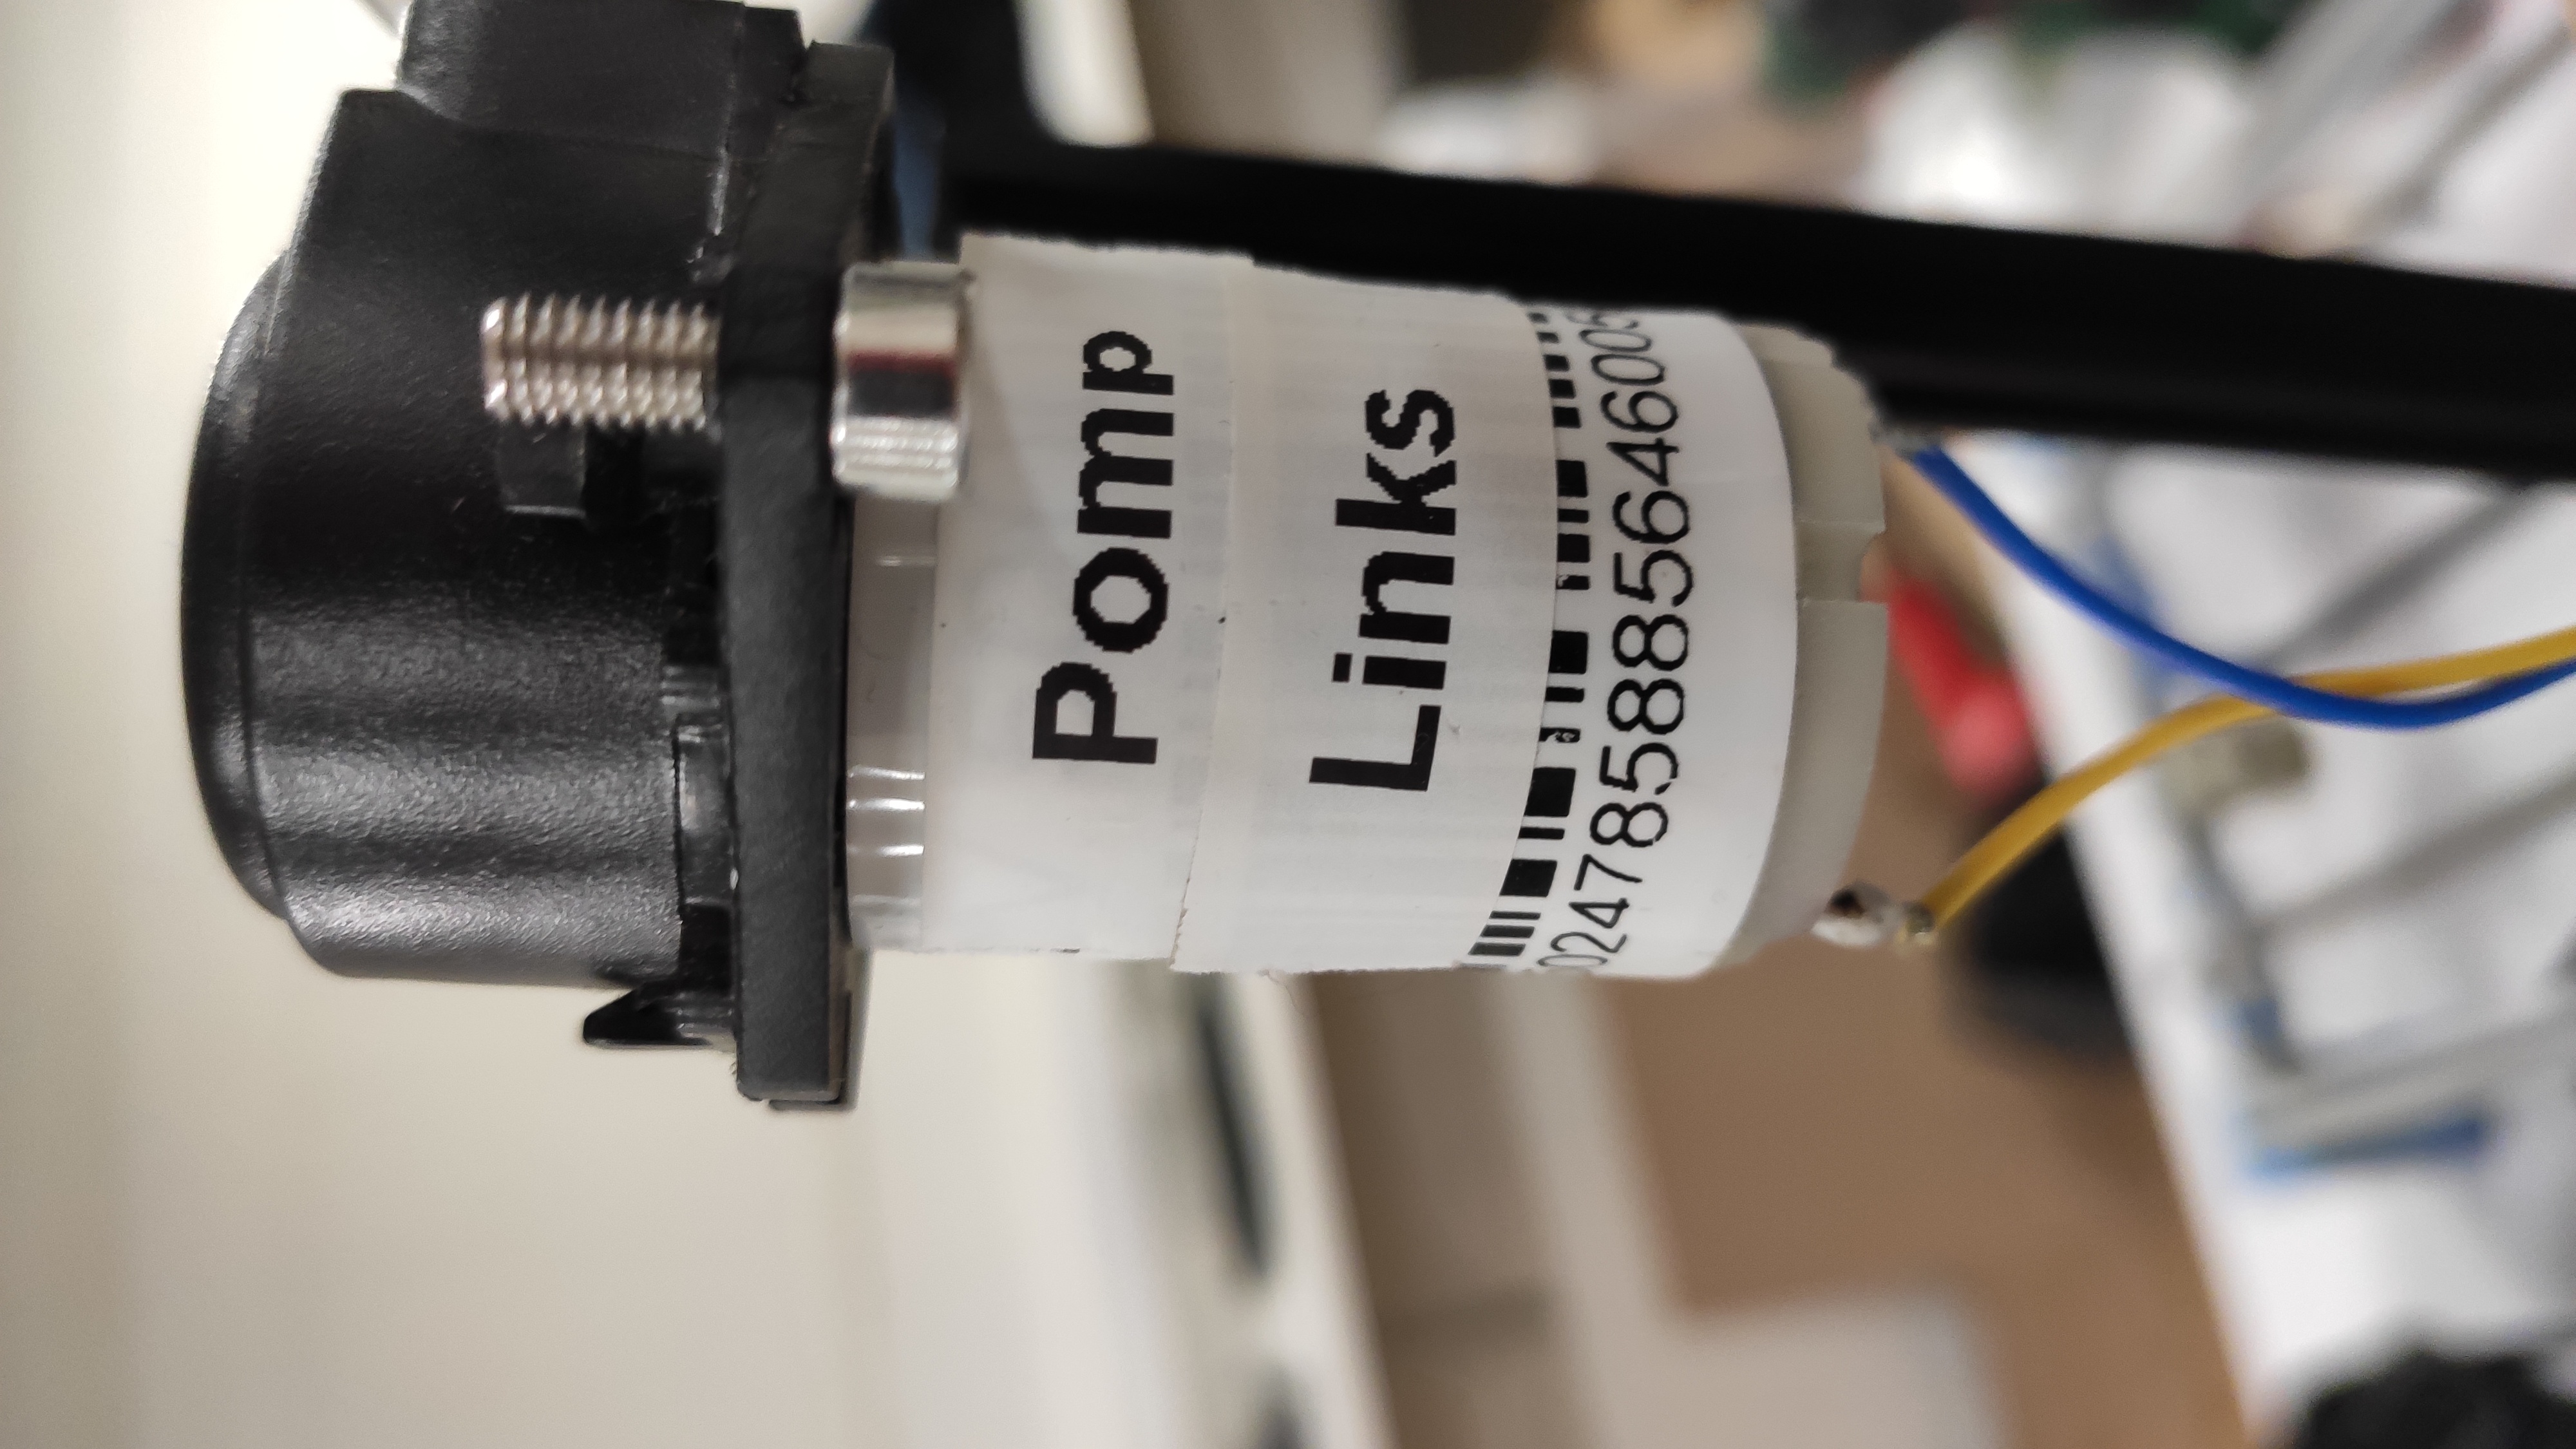
\includegraphics[width=\linewidth, angle=270]{pompLinks.jpg}
		\caption{Linkerpomp}
		\label{fig: linkerpomp}
	\end{minipage}%
	\begin{minipage}{.5\textwidth}
		\centering
		\includegraphics[width=\linewidth,angle=270]{pompRechts.jpg}
		\caption{Rechterpomp}
		\label{fig: rechterpomp}
	\end{minipage}
\end{figure}

\begin{figure}[h]
	\centering
	\includegraphics[width=0.5\textwidth,angle=270]{uiteindenLeidingen.jpg}
	\caption{Uiteinde leiding}
	\label{fig: uiteinde leiding}
	
\end{figure} 

\begin{figure}[h]
	\centering
	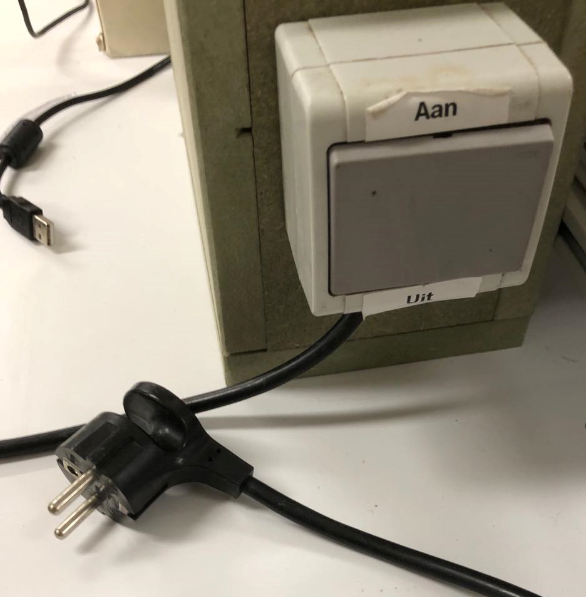
\includegraphics[width=0.5\textwidth]{stekker.png}
	\caption{Zwarte stekker}
	\label{fig:stekker}
	
\end{figure} 


\chapter*{Opstarten}
\label{hoofdstuk opstarten}
\section*{Opstarten van de microcontroller}
Om de automatic microplate dispenser op te starten, plaatst men de stekker in een wandcontactdoos en brengt men de schakelaar aan de groene box in de 'Aan'-positie (zie Figuur \ref{fig:schakelaar}, zorg er zeker voor dat het scherm en de muis verbonden zijn aan de microcontroller zoals beschreven in \ref{sectie hardware}).

\begin{figure}[h]
	\centering
	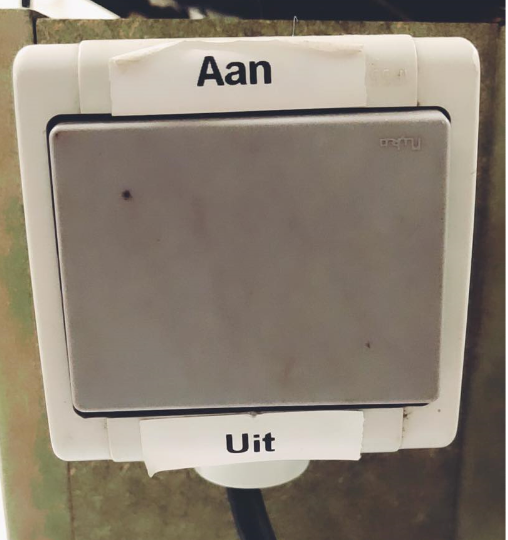
\includegraphics[width=0.5\textwidth]{schakelaar.png}
	\caption{Schakelaar in 'Aan'-positie}
	\label{fig:schakelaar}
	
\end{figure} 
Vervolgens wacht men enkele ogenblikken tot het startscherm van de automatic microplate dispenser verschijnt op het computerscherm. Vooraleer dit zal gebeuren, verschijnt er witte code op het zwarte scherm, dit is volledig normaal. Dit kan enkele ogenblikken duren. De microcontroller is volledig opgestart op het moment dat de grafische interface (zie Figuur \ref{fig: GI_letters1}) op het scherm komt.
 
\begin{figure}[h]
	\centering
	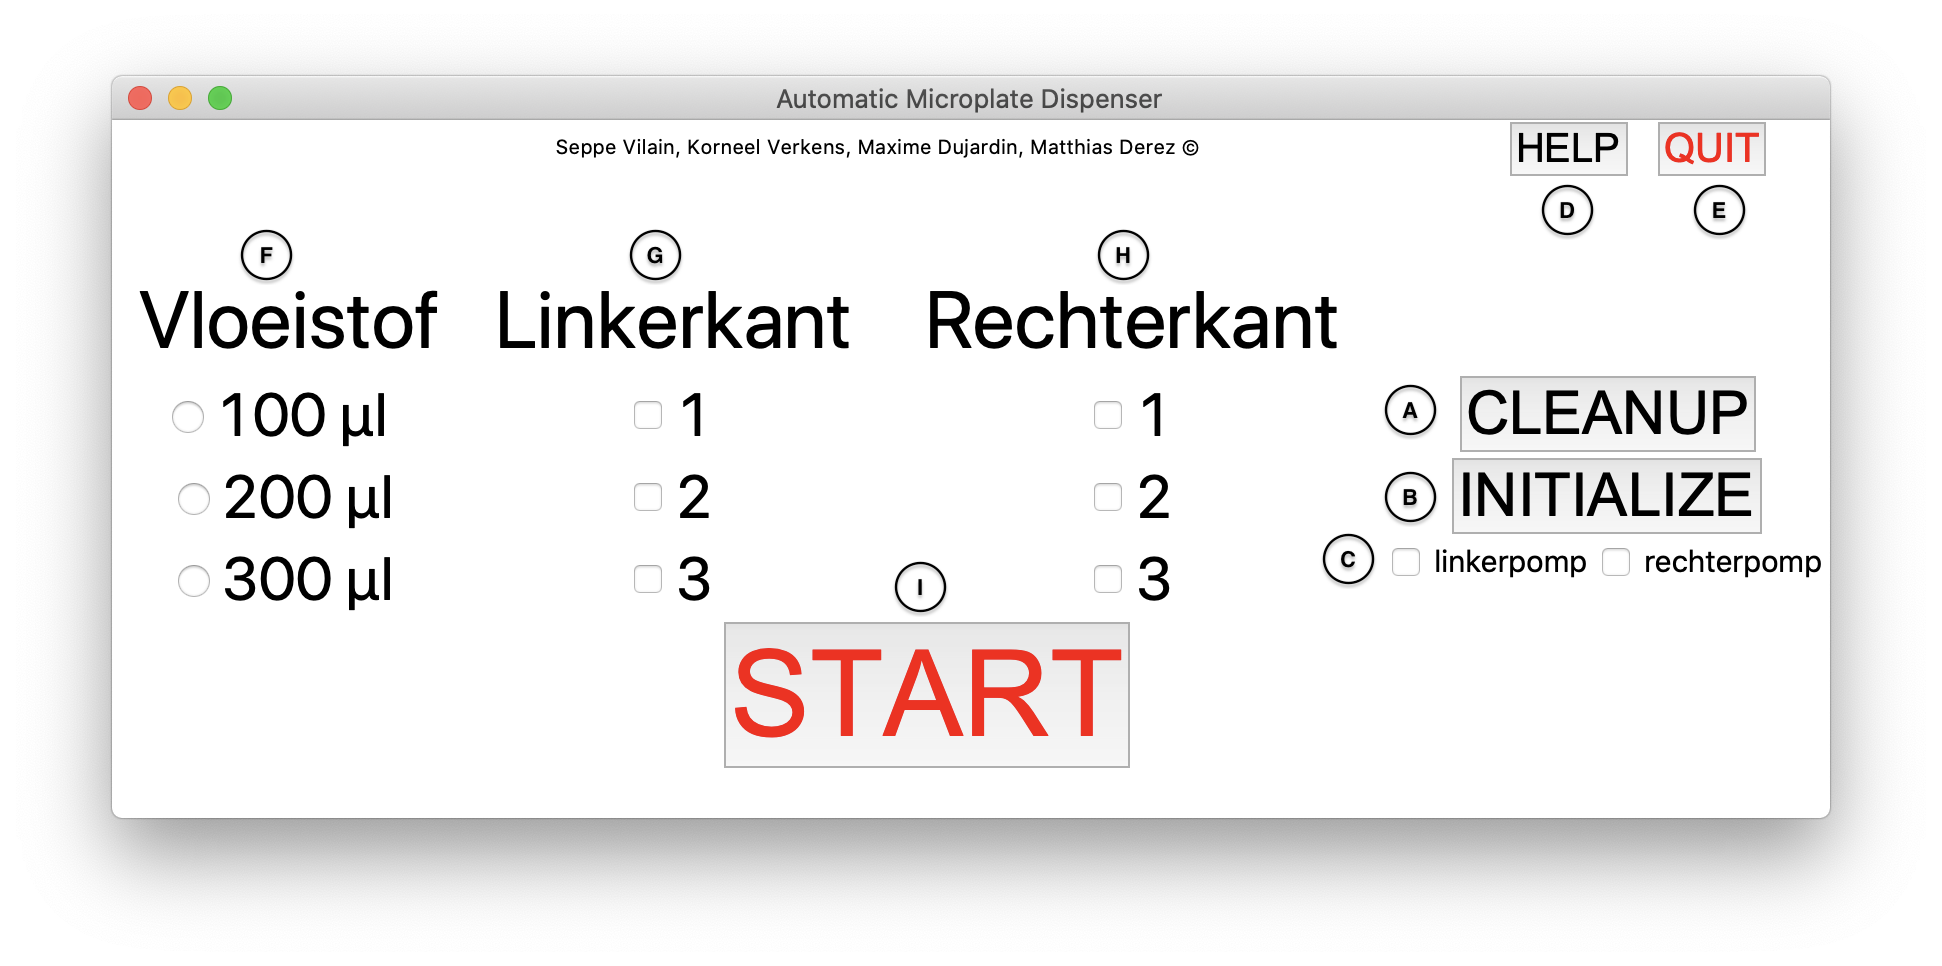
\includegraphics[width=1\textwidth]{GI_letters.png}
	\caption{Grafische interface}
	\label{fig: GI_letters1}
	
\end{figure} 

\section*{Opstarten van de machine}
\label{sec:initialize}

Vervolgens moet de machine geïnitialiseerd worden: de leidingen van het toestel worden hierbij gevuld met de vloeistof uit de erlenmeyers. Om dit te doen klikt vinkt men aan welke pompen geïnitialiseerd moeten worden (zie 'C' in Figuur \ref{fig:GI_letters}) en vervolgens op de knop 'INITIALIZE' (zie 'B' in Figuur \ref{fig:GI_letters}). Men kan kiezen om maar één van de twee pompen te initialiseren of om beide te initialiseren. Tijdens het initialiseren is het zeer waarschijnlijk dat er vloeistof uit de pipetpunten (zie Figuur \ref{fig: pipetpunten}) komt, het is dan ook aangeraden om een recipiënt onder de pipetpunten te plaatsen waarin deze vloeistof kan worden opgevangen. \\
Eens het toestel geïnitialiseerd is, is hij klaar voor gebruik. 

\begin{figure}[h]
	\centering
	\includegraphics[width=1\textwidth]{pipetpunten.jpg}
	\caption{Pipetpunten}
	\label{fig: pipetpunten}
	\end{figure} 


\chapter*{Uitvoeren test}

Nu de machine klaar volledig klaar is, kan men de ELISA-test uitvoeren. \\ \\
Men onderneemt hiervoor volgende stappen (de werkwijze wordt geïllustreerd via Figuur \ref{fig:GI_letters}):
\begin{enumerate}
	\item Selecteer de gewenste hoeveelheid vloeistof die in elke \textit{microwell} dient terecht te komen. Vink hiervoor 100 $\mu l$, 200 $\mu l$ of 300 $\mu l$ aan (zie 'F'). Let op: het is niet mogelijk om voor elke microplate een andere hoeveelheid te selecteren. Indien men dit vergeet te doen en de machine probeert te starten, zal een foutmelding op het scherm verschijnen.
	\item Selecteer op welke plaatsen microplates staan die gevuld moeten worden. Dit doet men door de nodige posities in 'G' en 'H' aan te vinken. Het is aan te raden om de te vullen microplates op zo laag mogelijke posities te plaatsen: op die manier zal het vullen van de microplates minder tijd in beslag nemen. Verifieer vooraleer op 'START' te klikken dat de microplates op de juiste posities staan.
	\item Klik op 'START' (zie 'I').  
\end{enumerate}

\chapter*{Afsluiten}

\section*{Afsluiten van de machine}
\label{sec:cleanup}

Om het apparaat af te sluiten moet men enkele stappen overlopen. Eerst en vooral is het noodzakelijk om de resterende vloeistof in de leidingen te verwijderen. Hiervoor klikt men op de knop 'CLEANUP' (zie 'A' in Figuur \ref{fig:GI_letters}). Alvorens dit te doen, dient men de uiteinden van de leidingen uit de erlenmeyer met de te onderzoeken vloeistof te halen (anders wordt er opnieuw vloeistof in de leidingen gezogen).


 Ook hier is het aan te raden om een recipiënt onder de pipetpunten te plaatsen, zodat de resterende vloeistof kan opgevangen worden. In de volgende stap wordt uitgelegd hoe de microcontroller uitgeschakeld kan worden.
 
 
\section*{Afsluiten van de microcontroller }
 
Het apparaat afsluiten doet men door op de knop 'QUIT' te klikken (zie 'E' in Figuur \ref{fig:GI_letters}). Het enige wat nog moet gebeuren is de machine afsluiten van de netstroom, dit doet men door de schakelaar \ref{fig:schakelaar} op 'Uit' te zetten (zie Figuur \ref{fig:schakelaar}). Als men het toestel wil verplaatsen, moet de stekker \ref{fig:stekker} ook verwijderd worden uit de wandcontactdoos. 

\chapter*{Grafische interface}

In dit hoofdstuk wordt nog een overzicht gegeven van de functies in de grafische interface. 

\begin{figure}[h]
	\centering
	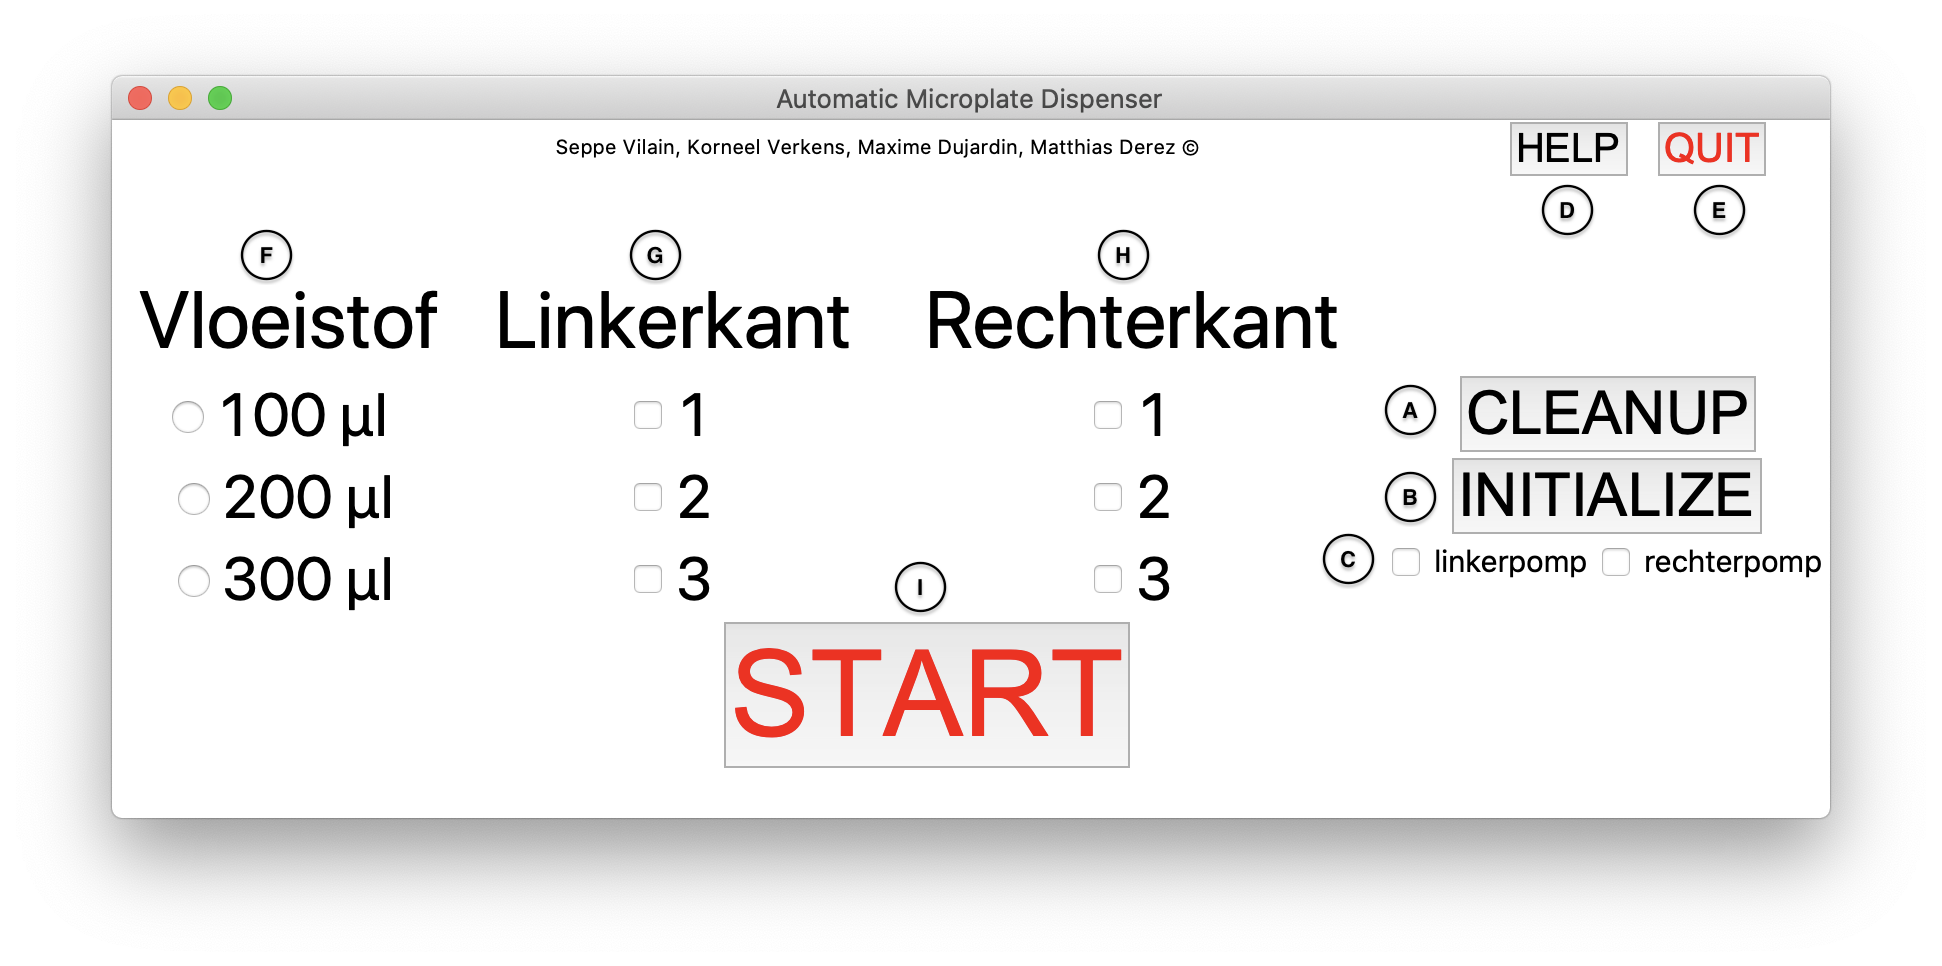
\includegraphics[width=1.2\textwidth]{GI_letters}
	\caption{Grafische interface}
	\label{fig:GI_letters}
\end{figure}

\begin{itemize}
	\item[A] Deze knop zorgt voor de \textit{cleanup} van het toestel. De methode om de leidingen te reinigen staat beschreven in \ref{sec:cleanup}.
	\item[B] Met deze knop wordt het apparaat geïnitialiseerd. Een beschrijving hiervan staat in \ref{sec:initialize}.
	\item[C] Hier kunnen de pompen geselecteerd worden die een bepaalde opdracht (initialisatie of cleanup) moeten uitvoeren. Men kan ofwel de linker- ofwel de rechterpomp ofwel beide pompen selecteren. 
	\item[D] Deze functie geeft kort weer hoe de machine kan opgestart worden.
	\item[E] Door op deze knop de klikken kan de automated microplate dispenser afgesloten worden.
	\item[F] Men kiest de hoeveelheid vloeistof per microwell door de juiste hoeveelheid aan te vinken.
	\item[G] Hier kiest men op welke posities van de linkerkant van de transportplaat microplates geplaatst zijn die gevuld moeten worden. 
	\item[H] Hier kiest men op welke posities van de rechterkant van de transportplaat microplates geplaatst zijn die gevuld moeten worden.
	\item[I] Dit is de knop die het initialiseren, cleanup en vullen van de microplates start.
\end{itemize}



\chapter*{Mogelijke problemen}
In dit hoofdstuk worden mogelijke problemen opgesomd met oplossingen.
\begin{enumerate}
	\item Het kan zijn dat er bij het einde van het initialiseren nog geen vloeistof uit alle pipetpunten komt. Wanneer dit voorvalt, kan men het toestel gewoon opnieuw initialiseren zoals eerder beschreven.
	\item Hetzelfde kan voorvallen bij de cleanup: het kan zijn dat bij het einde van de cleanup nog niet alle vloeistof uit de leidingen is. Dit kan opgelost worden door de cleanup opnieuw uit te voeren. 
	\item Wanneer de transportplaat bij het verplaatsen ergens hapert, dient men het toestel onmiddellijk uit te zetten. Vervolgens moet gekeken worden of er geen onzuiverheden tussen de lagers en de staven zitten. Indien dit het geval is, maak dan de staven schoon.
	\item Indien het toestel niet wil opstarten, controleer dan of de schakelaar van het toestel in de 'Aan'-positie staat en de stekker in het stopcontact zit. 

\end{enumerate}




\chapter*{Onderhoud} 

\section*{Pipetpunten vervangen}

De pipetpunten kunnen vervangen worden door de zwarte handschroeven (zie Figuur \ref{fig: handschroef})los te draaien. Vervolgens haalt men de huidige pipetpunten van het toestel en plaatst men de nieuwe pipetpunten op het toestel. Tot slot worden de handscroeven terug aangedraaid. 

\begin{figure}[h]
	\centering
	\includegraphics[width=1\textwidth,angle=270]{handschroef.jpg}
	\caption{Handschroef}
	\label{fig: handschroef}
\end{figure}

\section*{Leidingen reinigen}

De leidingen kunnen gereinigd worden door de uiteinden van de leidingen in een recipiënt met water te plaatsen. Vervolgens klikt men op de knop 'INITIALIZE' en vervolgens op de knop 'CLEANUP' op de grafische interface. Zorg er zeker voor dat er een recipiënt onder de pipetpunten staat.




\end{document}